\documentclass[12pt,a4paper,fleqn]{article}
\title{Progress Report}
\author{Syed Ahmad Raza}
\date{2016.12.27}
\usepackage{mathtools}
\usepackage{graphicx}
\usepackage{color}          % for color eps output
\usepackage{afterpage}
%\usepackage{layouts}       % for: \printinunitsof{in}\prntlen{\textwidth}

\begin{document}
\maketitle
\section*{Numerical solution for 2D heat transfer using unequally spaced
intervals and its comparison with analytical solution}

Heat transfer in a 2D block of pure silver (99.9\%) is considered. The equation
for unsteady heat transfer is as follows:

\begin{equation}
\frac{\partial T}{\partial t} = \alpha\left(\frac{\partial^2T}{\partial x^2} +
\frac{\partial^2T}{\partial y^2}\right)
\end{equation}

Two different sets of boundary conditions were analyzed. For the first case, the
analytical and numerical solutions were computed and compared. For the second
set of boundary conditions, only the numerical solution was computed. The
numerical solutions for both cases were computed until steady state was
achieved.

All the codes were written in C++ and all the plots were generated through
Matplotlib. $50 \times 50$ grids were used with unequal intervals selected for
their suitability to the solution.

\subsection*{Grid generation for unequally spaced intervals}
To practice grid generation with unequally spaced intervals, the following
function was used to generate the x-coordinates:
\begin{equation}
f(x)=L\sin\left(\frac{\pi}{L}\times\frac{i}{n_x}\right)
\end{equation}
where $L$ is the length of the block, $i$ is the index of the coordinate and
$n_x$ is the total number of intervals on the axis. The same function was
also used for the y-coordinates, with the necessary replacements of
variables. The resulting grid is shown in the figure below.

\afterpage{
\begin{figure}[t!]
\centering
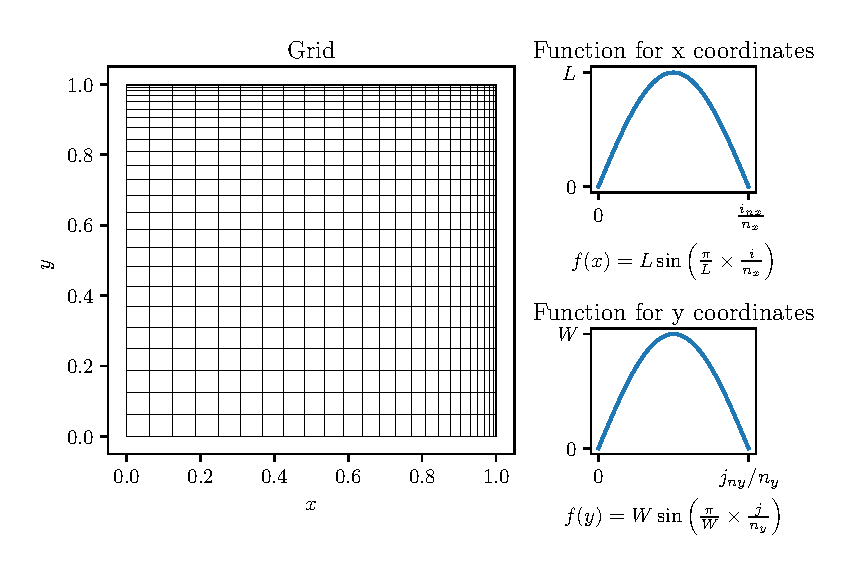
\includegraphics[width=\linewidth]{gridSimple.eps}
\caption{Practice grid with $x$ and $y$ functions and their graphs.}
\end{figure}
}

\newpage

\subsection*{First case}

The boundary conditions for this case have been selected as follows:

\begin{enumerate}
\item $T_{xi}=25^{\circ}C$ at $x=0$
\item $T_{xf}=25^{\circ}C$ at $x=L$
\item $T_{yi}=25^{\circ}C$ at $y=0$
\item $T_{yf}=50^{\circ}C$ at $y=L$
\end{enumerate}

\subsubsection*{Analytical solution for first case}

The simplified governing equation for the steady state reduces to:
\begin{equation}
\frac{\partial^2T}{\partial x^2} + \frac{\partial^2T}{\partial y^2} = 0
\end{equation}

The analytical solution to this problem is given by:
\begin{equation}
T(x, y) =
\frac{2T_3}{\pi}\sum\limits_{n=1}^{\infty}\left[\frac{(-1)^{n+1}+1}{n}\right]
\frac{\sin\lambda_nx\sinh\lambda_ny}{\sinh\lambda_nW} + T_1\end{equation}
where
\begin{equation}
\lambda_n = \frac{n\pi}{L}\quad\text{for}\quad n = 0, 1, 2, \ldots 
\end{equation}

The temperatures in this equation are defined as:
\begin{equation}
T_1 = T_{xi} = T_{xf} = T_{yi} \quad\text{and}\quad T_3 = T_{yf} - T_1
\end{equation}

The analytical solution was computed for $n = 1$ to $n = 200$. The results are
shown in the figure below.

\begin{figure}[b!]
\centering
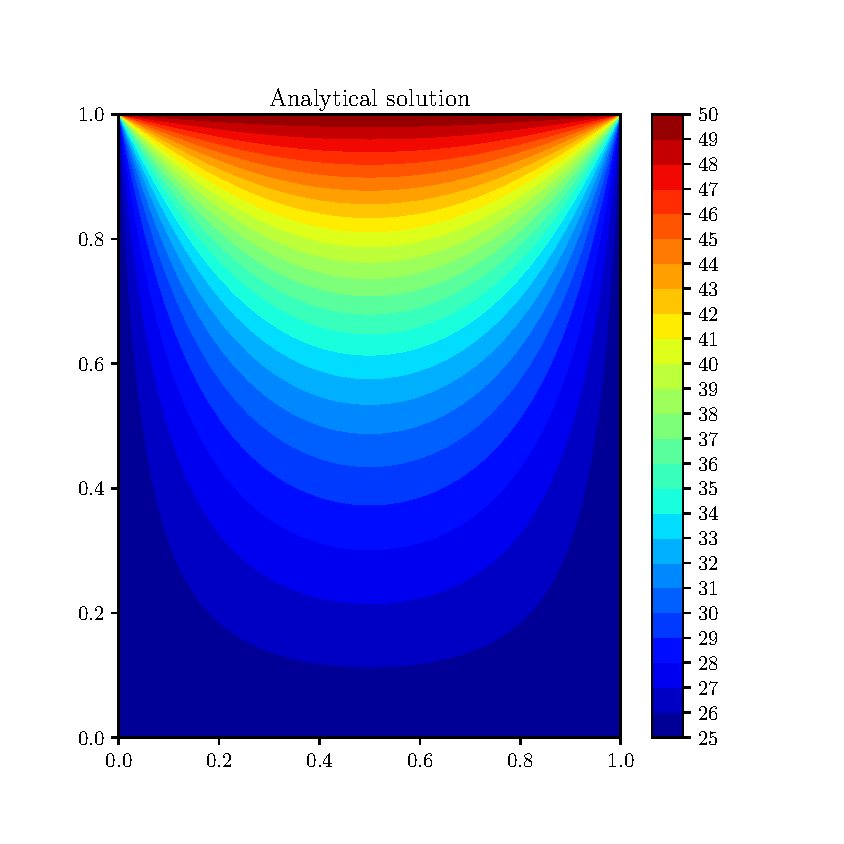
\includegraphics[width=\linewidth]{ht2dCase01Analytical.eps}
\caption{Plot for the analytical solution of case 1.}
\end{figure}

\newpage

\subsubsection*{Numerical solution for first case}

A C++ code was written for numerical solution of this unsteady 2D heat transfer
problem. Initial condition was $T_i=25^{\circ}C$ throughout the block.

A time step of 0.001 was utilized. A $50\times50$ grid was selected with the
following functions for the x and y axes:

\begin{equation}
f(x)=\frac{L}{2}\left[ 1 + \sin\left(\pi\left(\frac{i}{n_x} -
\frac{1}{2}\right)\right)\right]
\end{equation}
\begin{equation}
f(y)=W\sin\left(\frac{\pi}{2}\times\frac{j}{n_y}\right)
\end{equation}

These functions were selected so that a denser mesh could be obtained in areas
of the block where a larger temperature gradient is expected, from analysis of
the analytical solution. The resulting grid is shown in the figure below.

\begin{figure}[hp!]
\centering
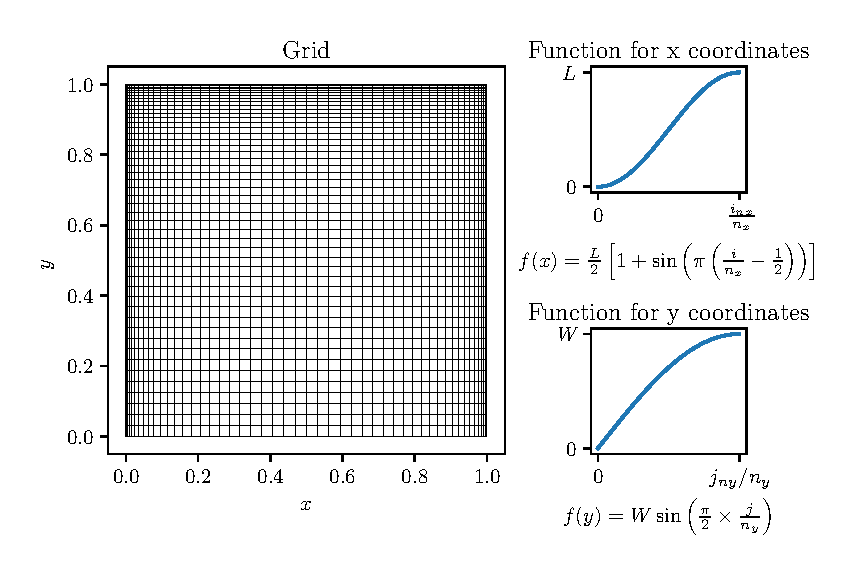
\includegraphics[width=\linewidth]{gridCase01.eps}
\caption{Grid for first case with $x$ and $y$ functions and their graphs}
\end{figure}

The following formula for forward in time, center in space method (FTCS) was
derived and used:

\begin{equation}
\begin{split}
\left.\frac{d^2f}{dx^2}\right|_i = \quad &\frac{2(f_{i+1} + f_{i-1}) -
4f_i}{(x_{i+1} - x_i)^2 + (x_{i-1} - x_i)^2}
\\& - \frac{2(f_{i+1} - f_{i-1})(x_{i+1} - 2x_i + x_{i-1})}{(x_{i+1} -
x_{i-1})[(x_{i+1} - x_i)^2 + (x_{i-1} - x_i)^2]}
\end{split}
\end{equation}

The root mean square difference was calculated at $x = L/2$ for all $y$ values
between successive iterations of time to determine the steady state, using the
following formula:
\begin{equation}
\text{RMS Difference} =
\sqrt{\frac{\sum\limits_{y=0}^{y_{n+1}}(T_{i-1}-T_i)^2}{n+1}}
\end{equation}
Steady state, assumed when RMS difference $\leq1\times10^{-10}$, was achieved at
$t=3741.219$ seconds.
The numerical solution was also compared with the analytical solution. The root
mean square difference (determined using the above formula) between the 
analytical and numerical solution was computed at $x = L/2$ for all $y$ values.
The result was found to be $0.00900^{\circ}C$.

The results for four time conditions, including the steady state, are shown
below.

\begin{figure}[p!]
\centering
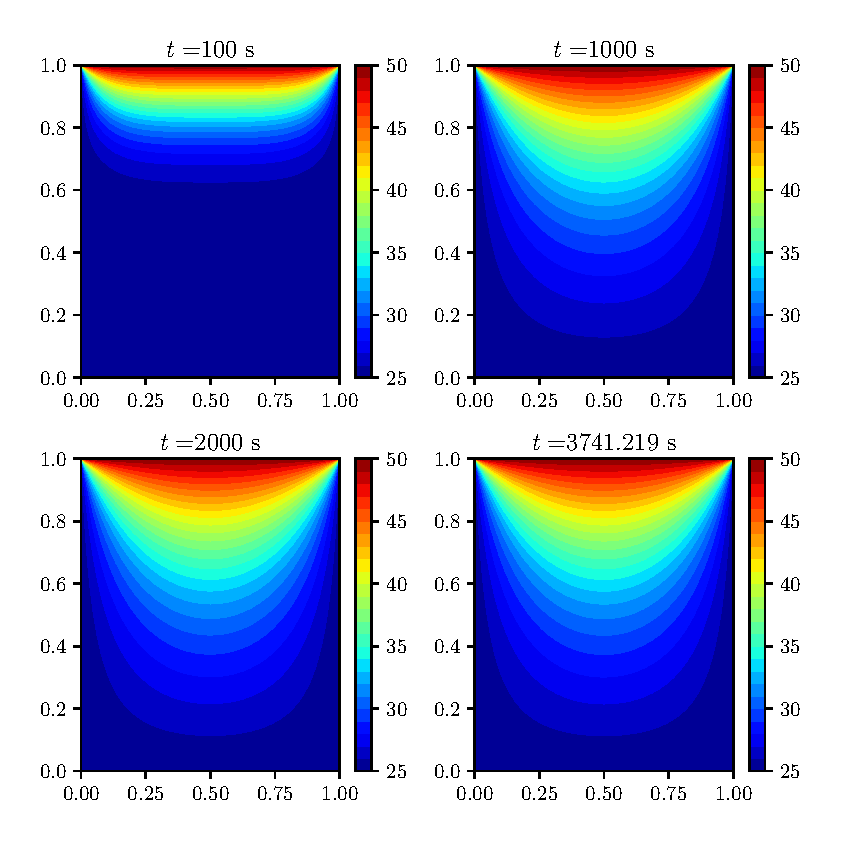
\includegraphics[width=\linewidth]{ht2dCase01.eps}
\caption{Plots for first case at various values of time (time step of 0.001).}
\end{figure}

\newpage

\subsection*{Second case}

The boundary conditions for the second case were selected as follows:

\begin{enumerate}
\item $T_{xi}=25^{\circ}C$ at $x=0$
\item $T_{xf}=50^{\circ}C$ at $x=L$
\item $T_{yi}=25^{\circ}C$ at $y=0$
\item $T_{yf}=50^{\circ}C$ at $y=L$
\end{enumerate}

\subsubsection*{Numerical solution for second case}

Again C++ code was written for numerical solution of this unsteady 2D heat transfer
problem. Initial condition was $T_i=25^{\circ}C$ throughout the block.

A time step of 0.001 was utilized. A $50\times50$ grid was selected with the
following functions for the x and y axes:

\begin{equation}
f(x)=L\sin\left(\frac{\pi}{2}\times\frac{i}{n_x}\right)
\end{equation}
\begin{equation}
f(y)=W\sin\left(\frac{\pi}{2}\times\frac{j}{n_y}\right)
\end{equation}

Again, the reason for selecting these functions was to achieve a denser
mesh in areas of the block having a larger temperature gradient, during the
intial time steps.
The resulting grid is shown in the figure below.

\afterpage{
\begin{figure}[hbt!]
\centering
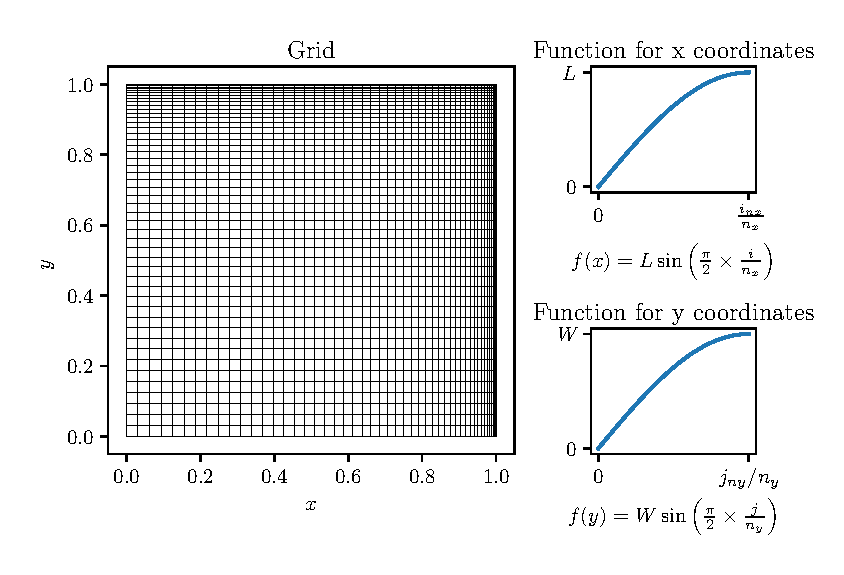
\includegraphics[width=\linewidth]{gridCase02.eps}
\caption{Grid for second case with $x$ and $y$ functions and their graphs}
\end{figure}
}

\newpage

The same formula used earlier for forward in time, center in space method (FTCS)
was utilized. The root mean square difference was calculated at $x = L/2$ for
all $y$ values between successive iterations of time to determine the steady
state.
Steady state, assumed when RMS difference $\leq1\times10^{-10}$, was achieved at
$t=3883.242$ seconds.

The results for four time conditions, including the steady state, are shown
below.

\begin{figure}[p!]
\centering
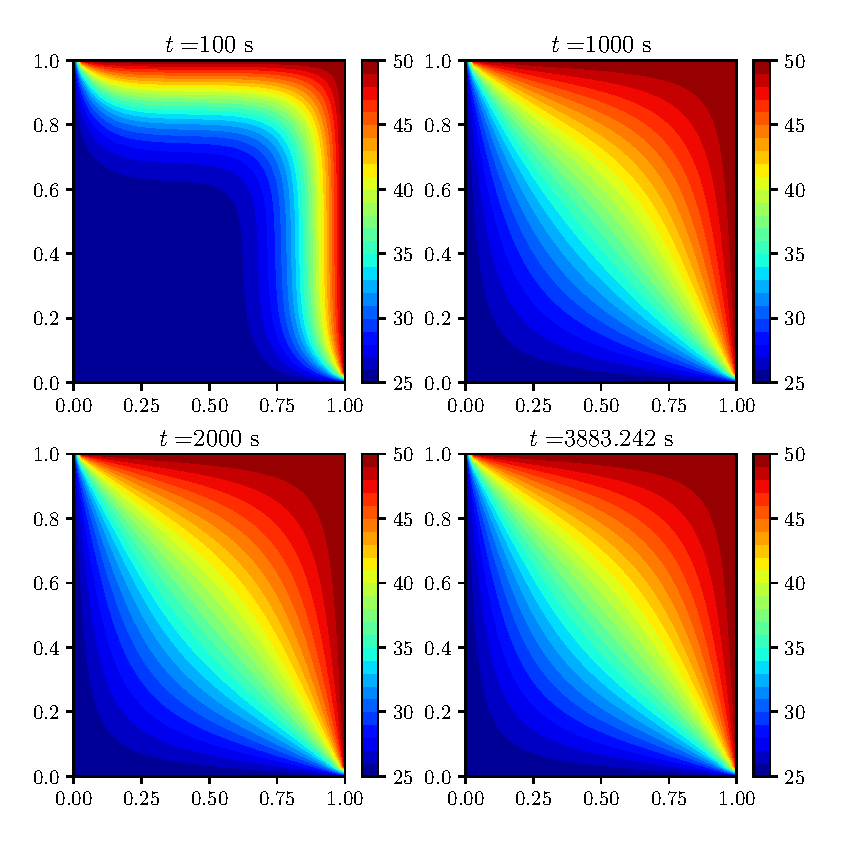
\includegraphics[width=\linewidth]{ht2dCase02.eps}
\caption{Plots for second case at various values of time (time step of 0.001).}
\end{figure}

\end{document}